% mainfile: ../Refinement.tex
\begin{figure}[h]
\centering
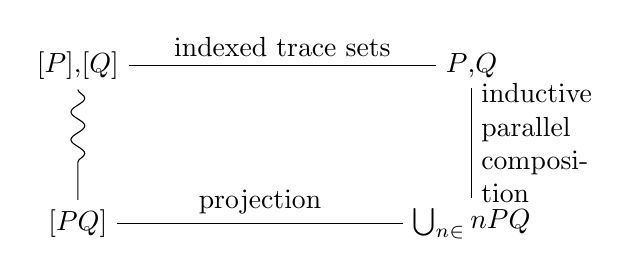
\begin{tikzpicture}
	\node   			(A)	{$\traces[P]$,$\traces[Q]$};
	\node[right of=A, xshift=40mm]	(B)	{$\trI{P}$,$\trI{Q}$};
	\node[below of=B, yshift=-10mm]		(C)	{$\bigcup_{n\in\N}\tracesI{n}{P}{Q}$};
	\node[below of=A, yshift=-10mm]		(D)	{$\traces[\procpar{P}{Q}]$};
	\path	(A)    edge node[anchor=south]  {indexed trace sets}            (B)
		(B)    edge node[anchor=west, text width=15mm]   {inductive parallel composition}    (C)
		(C)    edge node[anchor=south]  {projection}		(D);
	\path	(A)    edge[draw,decorate,decoration={snake, post=lineto, post length=4mm}] 
			    node[anchor=east]   {} (D);
\end{tikzpicture}
\caption{Visualization of the compositionality of the parallel operator (Part I).}
\label{fig_exp_comp_para}
\end{figure}
